% ------------------------------------------------------------------
\documentclass[12 pt]{article} % A4 paper set by geometry package below
\pagenumbering{arabic}
\setlength{\parindent}{10 mm}
\setlength{\parskip}{12 pt}

% Nimbus Sans font should be reasonably legible
\usepackage{helvet}
\renewcommand{\familydefault}{\sfdefault}
\usepackage[T1]{fontenc}  % Without this \textsterling produces $

% Section header spacing
\usepackage{titlesec}
\titlespacing\section{0pt}{12pt plus 4pt minus 2pt}{0pt plus 2pt minus 2pt}
\titlespacing\subsection{0pt}{12pt plus 4pt minus 2pt}{0pt plus 2pt minus 2pt}
\titlespacing\subsubsection{0pt}{12pt plus 4pt minus 2pt}{0pt plus 2pt minus 2pt}

\usepackage{amsmath}
\usepackage{amssymb}
\usepackage{graphicx}
\usepackage{verbatim}    % For comment
\usepackage[paper=a4paper, marginparwidth=0 cm, marginparsep=0 cm, top=2.5 cm, bottom=2.5 cm, left=3 cm, right=3 cm, includemp]{geometry}
\usepackage[pdftex, pdfstartview={FitH}, pdfnewwindow=true, colorlinks=true, citecolor=blue, filecolor=blue, linkcolor=blue, urlcolor=blue, pdfpagemode=UseNone]{hyperref}

% Put module code and last-modified date in footer
\usepackage{fancyhdr}
\pagestyle{fancy}
\fancyhf{}
\renewcommand{\headrulewidth}{0pt}
\cfoot{{\small \thisunit}\hfill \thepage\hfill {\small \moddate}}

% Hopefully address Canvas complaints about pdf tagging
%\usepackage[tagged]{accessibility}
\hypersetup {
  pdfauthor={David Schaich},
  pdftitle={Statistical Physics Tutorial Activity},
}
% ------------------------------------------------------------------



% ------------------------------------------------------------------
% Shortcuts
\newcommand{\De}{\ensuremath{\Delta} }
\newcommand{\la}{\ensuremath{\lambda} }
\newcommand{\lath}{\ensuremath{\la_{\mathrm{th}}} }
\newcommand{\Om}{\ensuremath{\Omega} }
% ------------------------------------------------------------------



% ------------------------------------------------------------------
\begin{document}
\newcommand{\thisunit}{MATH327 Tutorial (Mixing)}
\newcommand{\moddate}{Last modified 7 Mar.~2024}
\begin{center}
  {\Large \textbf{MATH327: Statistical Physics, Spring 2024}} \\[12 pt]
  {\Large \textbf{Tutorial activity \ --- \ Mixing entropy}} \\[24 pt]
\end{center}

This activity will be introduced in our 7 March tutorial, and you'll have the week until our next tutorial on 14 March to work on it.
In particular, we will discuss the mixing entropy in more detail in our next lecture on 8 March, after briefly summarizing the main concepts in the tutorial.
That brief summary will be enough for you to start working on the tasks below, given one assumption that we will justify in tomorrow's lecture.

Consider the thought experiment of starting with two canonical ideal gases, initially separated by a wall, each in thermodynamic equilibrium with $N$ particles in volume $V$ at temperature $T$.
We then remove the wall, allowing all $2N$ particles to mix in a $2V$ volume. % TODO: Go on about remaining in thermodynamic equilibrium?  Only relevant if $N_A \neq N_B$...
Finally, we re-insert the wall, dividing the $2N$ particles back into two re-separated subsystems.
It is safe to \textbf{assume} that $N$ particles end up in each of the two re-separated subsystems.
If we call these three stages $\{\Om_0, \Om_C, \Om_F\}$ with corresponding entropies $\{S_0, S_C, S_F\}$, we want to verify that $S_0 \leq S_C \leq S_F$ to obey the second law.

To do this verification, consider the specific setup shown by the figure below: \textit{All} $2N$ particles have identical physical properties, \textit{except} that those initially in the left compartment (the ``reds'') are distinguishable from those in right compartment (the ``blues'') by their colour.
After mixing and re-separation, red and blue particles can appear on either side of the wall in the final system $\Om_F$.

\begin{center}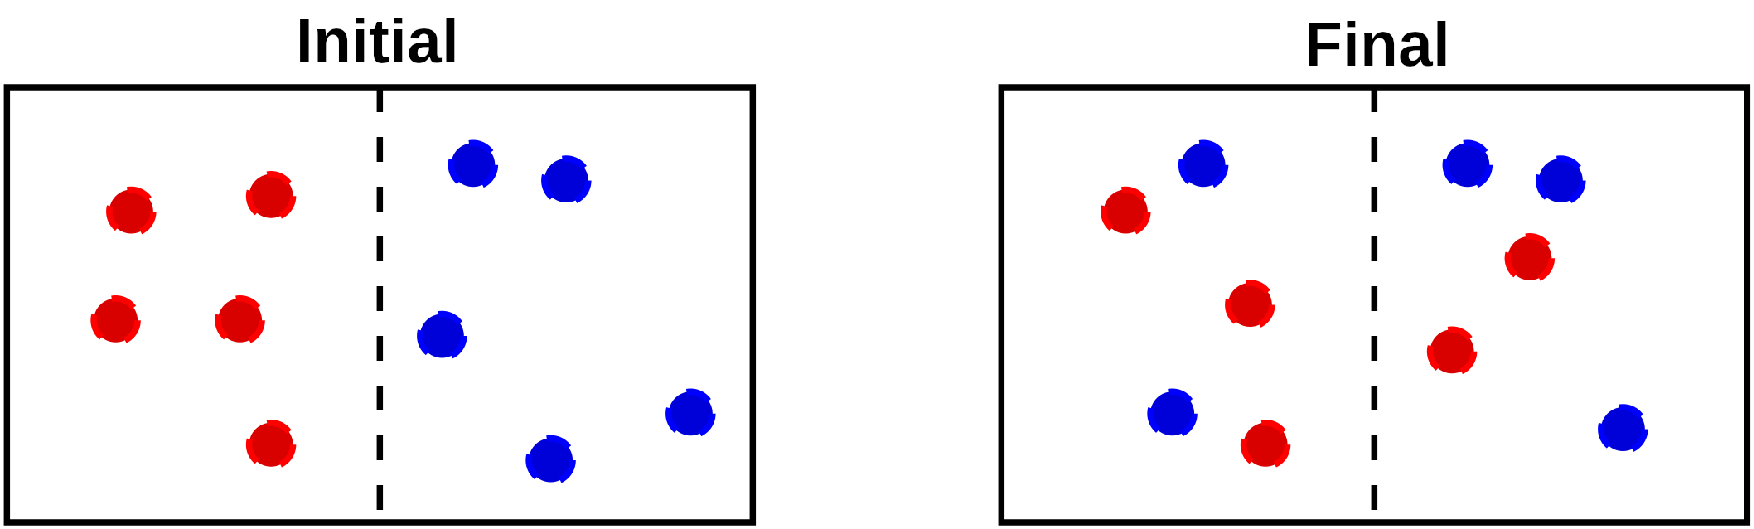
\includegraphics[width=0.8\textwidth]{figs/mix.pdf}\end{center}

\textbf{The first task} is to check $S_0 \leq S_C$ by computing both $S_0$ and $S_C$.
The difference $S_C - S_0 \equiv \De S_{\text{mix}}$ is the \textit{mixing entropy} that must be non-negative.
Since the combined system $\Om_C$ has two (distinguishable) sets of $N$ (indistinguishable) particles, its partition function is
\begin{equation*}
  Z_C = \frac{1}{N!} \frac{1}{N!} Z_1^{2N} = \frac{1}{N!} \frac{1}{N!} \left(\frac{2V}{\lath^3}\right)^{2N} \qquad \mbox{with} \qquad \lath = \sqrt{\frac{2\pi\hbar^2}{mT}},
\end{equation*}
where $Z_1 = 2V / \lath^3$ is the single-particle partition function.
It may be useful to exploit the properties of logarithms that connect differences of entropies to ratios of partition functions.

\newpage
\textbf{The second task} is to check $S_C \leq S_F$ by computing the final entropy $S_F$.
We can break this up into two steps.
The first of these is to compute the partition function $Z_F$ of the two re-separated systems (each with $N$ particles), summing over all ways of dividing the red and blue particles between them.
The following special case of the \href{https://en.wikipedia.org/wiki/Zhu_Shijie}{Zhu}--\href{https://en.wikipedia.org/wiki/Alexandre-Theophile_Vandermonde}{Vandermonde} \href{https://en.wikipedia.org/wiki/Vandermonde's_identity}{identity} for the \href{https://mathworld.wolfram.com/BinomialSums.html}{binomial sum} may be useful for this step:
\begin{equation*}
  \sum_{k = 0}^N \binom{N}{k}^2 = \binom{2N}{N}.
\end{equation*}
Finally, use your result for $Z_F$ to determine the final entropy $S_F$.
If you apply Stirling's formula, you may find it interesting to repeat your work with and without the $\log\left(\sqrt{2\pi N}\right)$ terms.

\end{document}
% ------------------------------------------------------------------
